
\documentclass[12pt]{article}
\usepackage{tikz}
\usepackage{geometry}

\usetikzlibrary{mindmap}

\author{ supercentinel }
%2019-01-01
\geometry{landscape, margin=1cm}

\begin{document}
\begin{center}
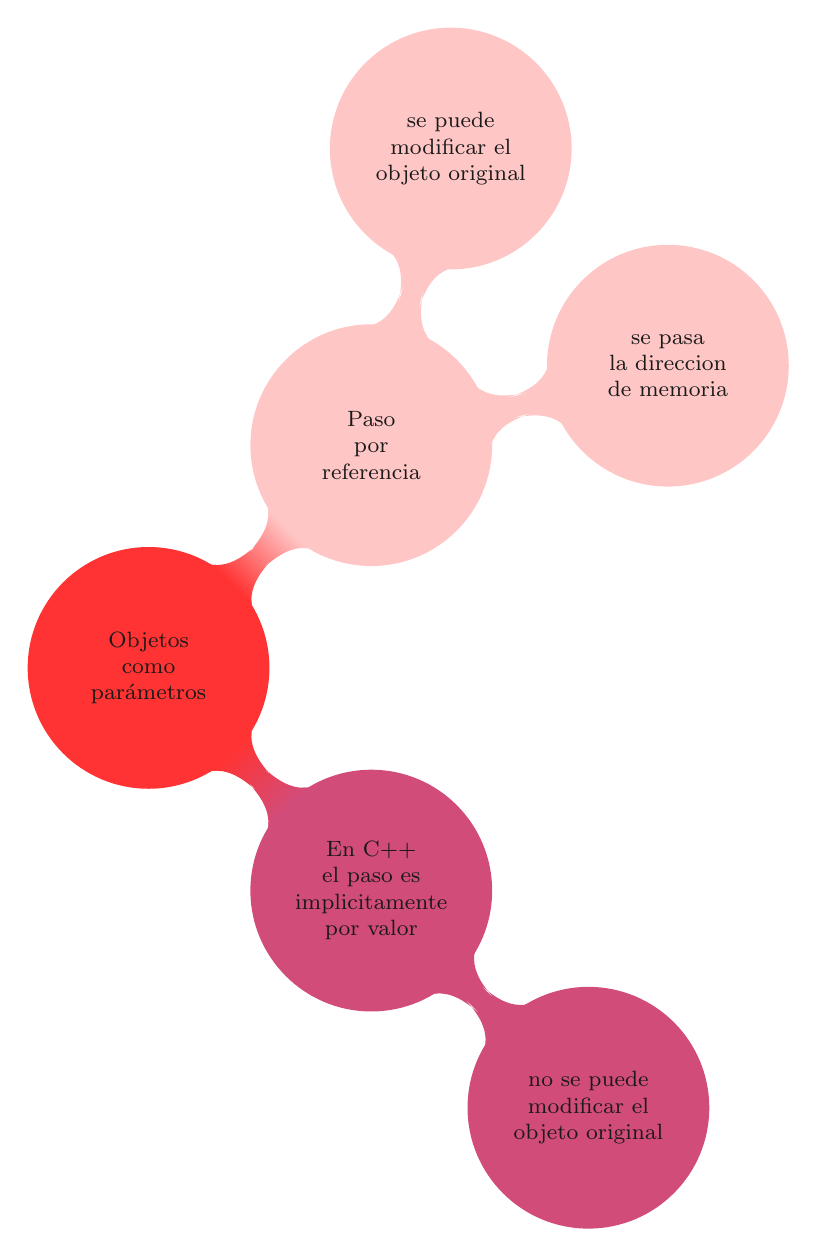
\begin{tikzpicture}[small mindmap, grow cyclic, every node/.style=concept,
    concept color=red!80, text=black!90, minimum size=3.0cm,
    level 1/.style={level distance=4.5cm,sibling angle=360/4},
    level 1/.style={level distance=4.0cm,sibling angle=360/4},
    level 2/.style={level distance=3.9cm,sibling angle=60},
    level 3/.style={level distance=3.5cm,sibling angle=60},
    ]
    \node{ Objetos\\como\\parámetros }
    child[concept color=purple!70] { node { En C++\\el paso es\\implicitamente por valor }
        child { node { no se puede\\modificar el\\objeto original } }
    }
    child[concept color=pink!90] { node { Paso\\por\\referencia }
        child { node { se pasa\\la direccion\\de memoria } }
        child { node { se puede\\modificar el\\objeto original } }
    }
    ;
\end{tikzpicture}
\end{center}
\end{document}
